\documentclass{article}

\usepackage{graphicx}
\usepackage{tikz}
\usepackage{tikzsymbols}
\usetikzlibrary{calc,patterns,shapes.geometric}
\pagestyle{empty}
\usepackage[margin=0pt]{geometry}
\geometry{papersize={14in,12in}}

\def\centerarc[#1](#2)(#3:#4:#5){\draw[#1] ($(#2)+({#5*cos(#3)},{#5*sin(#3)})$) arc (#3:#4:#5);}

\begin{document}
	\begin{figure}
		\centering
		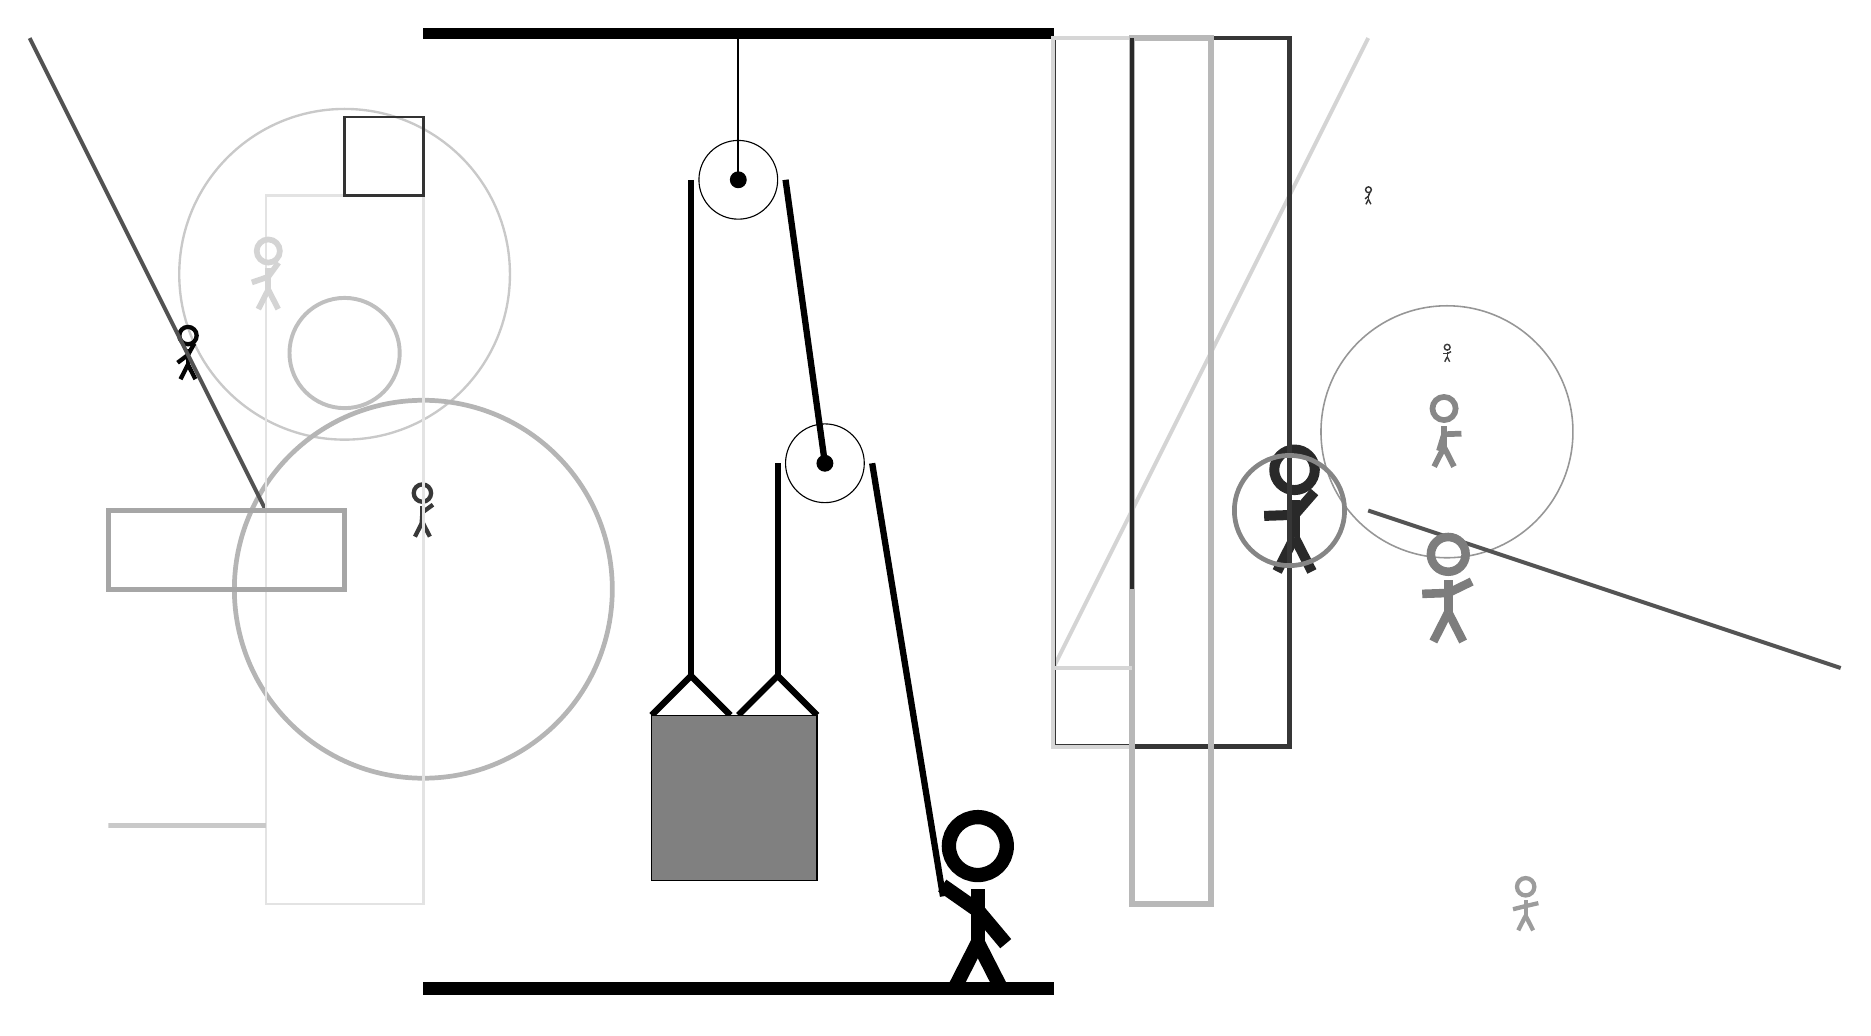
\begin{tikzpicture}
			%%%%% START %%%%%
			
			\draw[fill=black] (-2, 9) rectangle (6, 9.125);
			
			\draw (2, 7.2) circle (0.5);
			\draw[fill=black] (2, 7.2) circle (0.1);
			\draw[thick] (2, 7.2) -- (2, 9);
			
			\draw (3.1, 3.6) circle (0.5);
			\draw[fill=black] (3.1, 3.6) circle (0.1);
			
			\node[line width=0.2mm, color=black!84] at (9, 3) {\Strichmaxerl[7][2][49]};
			
			\node[line width=0.6mm, color=black!47] at (11, 4) {\Strichmaxerl[4][73][2]};
			\node[line width=0.6mm, color=black!77] at (11, 5) {\Strichmaxerl[1][0][28]};
			\draw[line width=0.5mm, color=black!17](6, 1) -- (10, 9);
			\draw[line width=0.6mm, color=black!79] (6, 0) rectangle (9, 9);
			\draw [line width=0.3mm, color=black!21](-3, 6) circle (2.1);
			\draw[line width=0.3mm, color=black!15] (7, 0) rectangle (7, -2);
			\draw [line width=0.6mm, color=black!29](-2, 2) circle (2.4);
			\node[line width=0.7mm, color=black!98] at (-5, 5) {\Strichmaxerl[3][37][61]};
			\draw[line width=0.5mm, color=black!68](-7, 9) -- (-4, 3);
			
			\node[line width=0.5mm, color=black!78] at (-2, 3) {\Strichmaxerl[3][86][36]};
			
			\draw[line width=0.3mm, color=black!11] (-2, -2) rectangle (-4, 7);
			\draw[line width=0.3mm, color=black!80] (-3, 7) rectangle (-2, 8);
			
			\draw [line width=0.2mm, color=black!41](11, 4) circle (1.6);
			\node[line width=0.6mm, color=black!39] at (12, -2) {\Strichmaxerl[3][14][13]};
			\node[line width=0.6mm, color=black!17] at (-4, 6) {\Strichmaxerl[4][19][54]};
			
			\draw [line width=0.5mm, color=black!25](-3, 5) circle (0.7);
			\draw[line width=0.7mm, color=black!21] (-4, -1) rectangle (-6, -1);
			\draw [line width=0.6mm, color=black!48](9, 3) circle (0.7);
			
			\draw[line width=0.5mm, color=black!16] (6, 0) rectangle (7, 9);
			\draw[line width=0.5mm, color=black!67](10, 3) -- (16, 1);
			\node[line width=0.6mm, color=black!51] at (11, 2) {\Strichmaxerl[6][2][26]};
			\node[line width=0.3mm, color=black!80] at (10, 7) {\Strichmaxerl[1][39][69]};
			\draw[line width=0.7mm, color=black!28] (8, 9) rectangle (7, -2);
			\draw[line width=0.5mm, color=black!16](6, 1) -- (7, 1);
			
			\draw[line width=0.5mm, color=black!84](7, 2) -- (7, 9);
			
			\draw[line width=0.6mm, color=black!35] (-3, 3) rectangle (-6, 2);
			
			\draw[line width = 0.8mm]  (0.9, 0.4) -- (1.4, 0.9) -- (1.9, 0.4);
			\draw[line width = 0.8mm]  (2.0, 0.4) -- (2.5, 0.9) -- (3.0, 0.4);
			\draw[fill=black!50] (0.9, 0.4) rectangle (3.0, -1.7);
			
			\draw[line width = 0.8mm] (1.4, 7.2) -- (1.4, 0.9);
			\centerarc[line width = 0.8mm](2, 7.2)(0:180:0.6);
			\draw[line width = 0.8mm] (2.6, 7.2) -- (3.1, 3.6);
			\draw[line width = 0.8mm] (2.5, 3.6) -- (2.5, 0.9);
			\centerarc[line width = 0.8mm](3.1, 3.6)(0:180:0.6);
			\draw[line width = 0.8mm] (3.7, 3.6) -- (4.6, -1.9);
			
			\node at (5, -2) {\Strichmaxerl[10][-35][-50]};
			
			\draw[fill=black] (-2, -3) rectangle (6, -3.15);
			
			%%%%% END %%%%%
		\end{tikzpicture}
	\end{figure}	
\end{document}